\documentclass[a4paper]{article}
\usepackage{a4wide}
\usepackage{url}
\usepackage{graphicx}
%\pagestyle{empty}

\def\META#1{\textit{${\cal MET\!\!A}$#1}}
\def\TODO#1{\texttt{\bf {TODO:} #1}}

\widowpenalty=10000
\clubpenalty=10000

\title{Virtualizing \META{Center} Resources Using Magrathea}
\author{Ji\v{r}\'\i{} Denemark \and Miroslav Ruda \and Lud\v{e}k Matyska}

\begin{document}

\maketitle

\begin{abstract}
Contemporary production grids do not usually offer the flexibility users are
looking for. While different user communities have often contradictory
requirements on the operating system, libraries, and applications, the
production Grids provide only one rigid environment. This rigidness can be
overcome by virtualization, when every user community or even individual user
can be provided with its own instance of a virtual Grid, running optimized and
tailored operating system and services. The promise of higher flexibility of
virtual Grids is compensated by the increase in scheduling complexity. In this
report, we present the Magrathea system that extends the Grid resource
management systems with support for virtual environment. After discussing the
design requirements, we introduce the Magrathea architecture that consists of
three components: the master and slave processes running on virtualized
resources and the cache process to provide the information about virtual
machine state to the scheduler. Two virtual machines sharing one physical
resource and used exclusively, preemption of a lower priority job running in a
virtual machine, support for more than two concurrently virtual machines
(domains) and support for ``frozen'' services that are repeatedly invoked and
suspended are the use scenarios discussed in the second part of the report. We
demonstrate how they are supported by the Magrathea system and what
modifications to the Grid resource management system are necessary. The
Magrathea is currently in the pre-production use on the Czech national Grid
environment \META{Center}. This report is an extended version of the paper
called ``Scheduling Virtual Grids: the Magrathea System'', which was presented
at VTDC~2007.
\end{abstract}

\section{Introduction}

Large-scale distributed computing and storage systems (Grids) already started
to be used by many scientific communities as indispensable tool supporting
their research. Successful Grid deployment attracts new communities, whose
computing requirements and patterns of use differ from the communities that
initiated the Grid development and deployment. Also, as Grids are an object of
intensive research and development, many middleware systems are deployed,
providing features that suit different user groups. 

Successful Grid deployment attracts also resource providers, who are
interested in providing new services and increasing both the number of users
and their satisfaction. However, they face a very difficult question of
selecting the ``right'' Grid, that would be adequate for majority of their
users and at least acceptable for the remaining ones. As the production Grid
environments like the EGEE have very strict requirements on the installed
operating system, libraries and the general system environment, it is very
difficult to merge this strict ``no-choice'' condition with the richness of
requirements of scientific communities. 

Apart from the differences in middleware (and implied operating system
requirements), the user communities also differ in their expectations of the
major Grid benefits. For the ``founding fathers'' (esp. the high energy
physics community) Grids are a place to store, share, and process enormous
amounts of data by rather simple (i.e., not highly parallel) jobs. On the
other hand, new users need support for large MPI jobs, require a fast
turn-around for short jobs or are looking to use Grids as a fabric to run
services whose use varies over time, i.e., the physical resources are not
efficiently used but this is a price for having a low reaction time when the
service is actually called. The best effort service, treating jobs as having
equal priority, is also not always sufficient and different priority schemes
are required by end users.

As the result of all these aspects, the current Grid production environments
are too restrictive for many potential users and the users are not motivated
enough to ``climb the wall'', although otherwise the benefit of sharing
computing resources and data among their collaborators is very attractive.

A potential remedy is to \emph{virtualize} the Grid environment. Through this
process users will get the illusion that they have access to a Grid which is
optimized to suit their particular needs. Precise versions and flavors of
operating system, libraries, middleware and application can be deployed with
virtual Grids without any unexpected interference with environments (other
virtual Grids) deployed for other user groups (or even for the same group but
for different application or its version). Building virtual Grids over Virtual
Machines (VM)~\cite{vmms} provides additional benefits to this concept. The
virtual machine provides almost ideal encapsulation of the whole operating
system and its components, including the Grid middleware. It can also be
optimized to serve a particular application (e.g., setting specific buffer
sizes, using non-standard libraries etc.).

The encapsulation provided by the virtual machine makes it rather easy to
offer additional services. It is reasonably easy to dynamically change the
basic physical resources (CPU, memory) allocated to the virtual machine. The
virtual machine can be easily checkpointed, it can be migrated to another
physical resource, the image stored for later inspection or re-run. Virtual
machines can be preempted, in a uniform way and without additional complexity
due to applications differing needs. While all these properties are best used
on a single machine (i.e., with parallelism limited to a single machine), the
support for large parallel jobs is not excluded.

Deploying virtual Grids, running on a low level physical fabrics, requires new
scheduling strategies and tools. Several virtual machines can run concurrently
on a single physical machine, the resources allocated to individual virtual
machines change in time, virtual machines may be checkpointed. All these new
features must be understood and taken care of by the Grid scheduling system.

To serve these needs, we have developed a system called Magrathea to allow
Grid job scheduling systems to deal with several virtual machines running on a
single computer and to submit correctly jobs into those VMs. Magrathea is
deployed in production environment on computational nodes of
\META{Center}\footnote{http://meta.cesnet.cz/}, which provides a computational
infrastructure for various groups of users with specific requirements and its
resources are also provided for European grid infrastructure
EGEE\footnote{http://www.eu-egee.org/}. 

\section{Magrathea System}
\label{sec:magrathea}

Scheduling in a virtual Grid environment depends on the way the virtualization
is understood. The simplest approach is to replace ``job'' with ``virtual
machine'', attach each job to its virtual machine and schedule whole virtual
machines in the same way as jobs. While simple and not requiring any complex
modifications to the scheduling system, this approach is also very limited in
using new features provided by virtual Grids. When deployed, it can also have
a substantial negative effect on the efficiency of the resource use. Starting
a job equals to booting a virtual machine (part of the overhead can be
mitigated using hibernated images, but still the startup latency my be rather
high). We decided to follow a different way, where the scheduler is at least
partially aware of the more complex environment of the virtual Grid and is
therefore able to deal with several virtual machines sharing the same physical
machine, with virtual machines that has been suspended, etc. The design
requirements we considered are presented in the next section, followed by the
Magrathea architecture description.

\subsection{Design Requirements}

When designing the Magrathea system we started with the following set of basic
requirements:

\begin{itemize}

\item There are more active (i.e., running) virtual machines than physical
resources. The resource management system must schedule jobs to these machines
exclusively, not overloading the resources.

\item As small as possible dependence on actual resource management system.
While currently used together with the PBS Pro, the dependence must be clearly
defined and new resource management systems easily supported.

\item No or just minimal modifications of the resource management system. This
complements the previous item on making Magrathea a universal system not tied
with a particular resource management system only, as this would limit the
usability of the Magrathea system.

\item Independence on system used for management of virtual machines (system
used for VM configuration, image preparation, booting etc.). Currently, we
support virtual machines started from pre-installed images, but we foresee
cooperation with some management system developed by other groups
(\cite{invigo,workspaces}).

\item Independence on particular VM implementation. 

\end{itemize}

To get better understanding of the relationship between Magrathea and the
resource management system we also devised three complementary use scenarios
that must be supported by the Magrathea system:

\begin{enumerate}

\item Exclusive use of the physical resource by one virtual machine at a time
while supporting concurrent active wait of several virtual machines on the
same resource.

\item Sharing one physical machine between several virtual machines running
concurrently and assigning of resources (CPUs, memory) to virtual machines
according requirements of jobs running in these virtual machines.

\item Support for preemption of virtual machines, eventually extended with
suspension and migration to different physical machine.

\end{enumerate}

To represent different states of virtual machines, we introduced the
\textit{Magrathea status} of virtual node. These new states are used to extend
the view of Grid as used by the resource management system (PBS Pro in our
case) for decisions made by the scheduler. The states are reported to the
resource management system directly by the concurrently running virtual
machines. However, the third scenario presented above requires further
adaptation, as the checkpointed virtual machine is not active and could not by
itself report its state. Thus, it is the responsibility of Magrathea
extensions to keep track of these virtual machines and to activate them when
necessary.

\subsection{Architecture} 

Magrathea system consists of three main components: master process
representing physical machines, slave processes running in each virtual
machine and optional cache process, storing information about status of all
virtual machines running on a cluster. Architecture of Magrathea and
interaction with resource management system and virtual machine monitor is
depicted in Figure~\ref{fig:architecture}.

\begin{figure}[tb]
    \begin{center}
    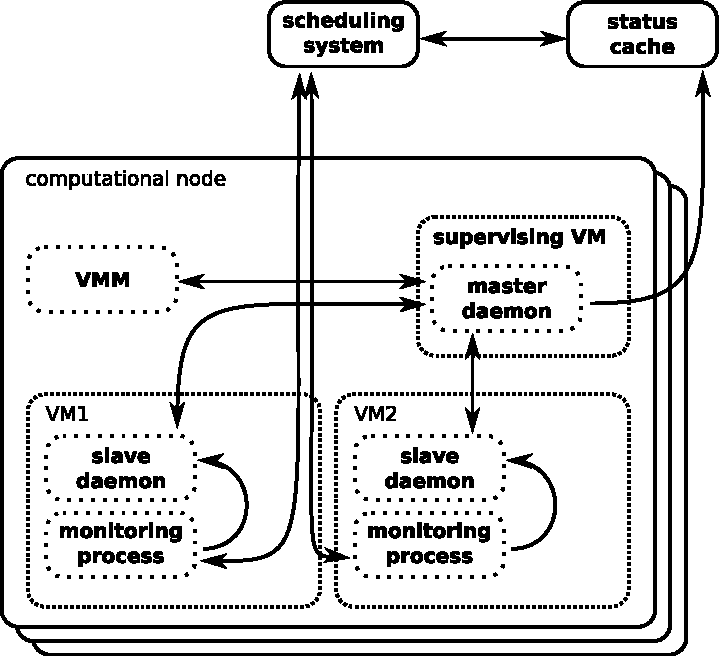
\includegraphics[width=.6\textwidth]{architecture}
    \end{center}
    \caption{The architecture of Magrathea}
    \label{fig:architecture}
\end{figure}

In the simplest use case scenario, when single-node job is started on a free
virtual machine, communication between resource management system and
Magrathea is as follows:

\begin{itemize}

\item When job appears in resource management system, it is task of the
\textit{scheduler} to select node where job should run. This part usually
includes getting information about the state of all queues and nodes and
selection of the node that fits best job requirements and has free resources
to run the job (the ``node'' can usually be a particular machine or a
head-node of a cluster with its local queue system). We do not modify this
behavior, we only extend the view of the Grid with which the scheduler is
working with information provided by Magrathea (to consider only virtual
machines ready to accept new jobs).

\item Magrathea runs its daemons in each virtual machine. A \emph{master}
daemon is run in the supervising Virtual Machine, to oversee all the virtual
machines deployed. The \emph{slave} daemon runs in each virtual machine, to
report its state to the master daemon. When job is submitted to the virtual
node, Magrathea slave daemon must be able to intercept this information. In an
ideal case, this is done before the job is actually started and slave contacts
the Magrathea master synchronously with the job submission.

\item The master recomputes status of all virtual machines and performs all
the necessary steps, for example, it assigns resources (CPU, memory) to the
virtual machine which will to run job. 

\item In rare cases, when the scheduler made its decision on a stale
information  or when the virtual machine state changed after the status
collection, the job may not be allowed to start. This is checked by the slave
process (it serves as a synchronization point in the case of race conditions)
and if a problem is encountered (i.e., the virtual machine is either in
non-accepting state or already running a different job), the startup is
interrupted and the job is returned to the scheduler to another submission
attempt.

\item When the job is finished, the slave notifies the master. The master
recomputes status of virtual machines supervised, changes mapping of resources
to virtual machines and prepares the node to accept new job(s).

\end{itemize}

More complex scenarios are described in the next section.

The master process, running in the supervising virtual machine, is responsible
for the management of virtual machines, their status recomputations, and
assignment of hardware resources to virtual machines. The master is also
responsible for reporting status information about all virtual machines to the
cache process. To achieve independence on a particular virtual machine
implementation, the master provides an interface to a virtual machine monitor
so that specific actions can be performed to activate and deactivate virtual
machines, change resources dedicated to specific virtual machine etc. In the
current implementation, master supports Xen~\cite{xen} and
VServer~\cite{vserver} virtualization systems.

Magrathea slave process has three main tasks:

\begin{itemize}

\item Report to the master when job is started or finished. This information
is used by the master when computing status of virtual machines. In the
current implementation, we use PBS Pro mechanism of prologue and epilogue
scripts, which are called when the job starts and finishes, respectively.

\item Accept commands from the running virtual machine (status query, suspend
command).

\item When notified by master, the slave starts scripts which must be run
inside the virtual machine (before or after domain is suspended or activated,
before and after domain is preempted etc.).

\end{itemize}

Cache service stores status information of virtual machines and related data
in a central database. This component is optional, it is not required when
resource management system is able to get Magrathea status information
directly from nodes. However, polling all worker nodes may slowdown resource
management system, therefore status cache may be used to improve performance
and scalability. We found that use of the status cache as the primary
information source for the PBS Pro scheduler not only for the Magrathea status,
but for other used metrics (otherwise obtained by polling either the PBS Mom
processes on nodes or other information services) improves the overall
responsiveness of the PBS Pro system. In the current implementation,
information about actual disk space usage and memory usage is pushed by
sensors from cluster nodes to the cache and this information is later used by
scheduler, too. We have also extended cache service to be able to aquire
(poll) information from Ganglia~\cite{ganglia} and PBS. Cache processes can
also form hierarchy of information services, cache can be configured to push
stored information to upper-level cache or acquire information from other
caches by polling.

\subsection{Two Static Domains}

In the first proposed scenario, several virtual machines (domains) are
deployed on one physical machine, but only one is allowed to run jobs in any
particular time. This active domain is provided with almost all resources (CPU
and memory in current implementation), while all remaining domains are also
running, but with minimal resources. Inactive domains are provided with
minimal percentage of CPU time, but they still behave like live domains for
resource management system---they send monitoring information to the
scheduler.

The individual states of each domain and their transition is depicted in
Figure~\ref{fig:twoVMs} for the case of two domains sharing one physical
resource. When the node is initiated, all domains start in the \emph{free}
state. In this state, the virtual machine is able to accept a job, changing
its state to \emph{running}. When one virtual machine becomes \emph{running},
all the resources are allocated to it and the state of all remaining domains
is changed to \emph{occupied}. If the \emph{running} domain does not need all
the resources (e.g., it requires only two cores on a four core machine), other
jobs can be send to the same domain (virtual machine). When all jobs that run
in a particular domain finish, all domains become \textit{free} again.

\begin{figure}[tb]
    \begin{center}
    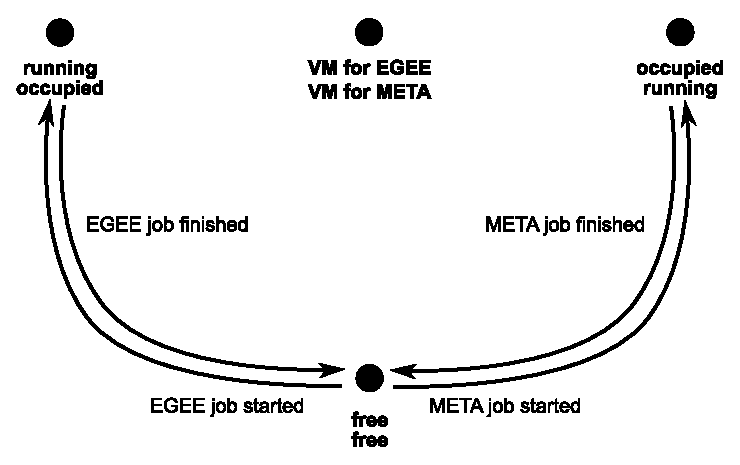
\includegraphics[width=.6\textwidth]{twoVMs}
    \end{center}
    \caption{States and transitions between them for statically deployed
        virtual machines.}
    \label{fig:twoVMs}
\end{figure}

In the current deployment on \META{Center}, sharing of worker nodes between
EGEE and \META{Center} is implemented using this setup. On each worker node,
two virtual machines providing \META{Center} and EGEE environments are
installed and running. In both virtual machines, standard \textit{PBS Mom}
(PBS monitoring daemon, which is responsible for job startup and monitoring,
but also for reporting node status to server) is running. While the same
architecture, number of CPUs etc. is published into \textit{PBS server},
different properties describing different installed environments are
published. This way, users may choose during submission whether they need
nodes with EGEE or \META{Center} environment. According to the user specified
properties, jobs are routed to appropriate EGEE or \META{Center} queues. It is
possible to distribute the cluster un-evenly between the two environments
using limits set on queues.

Some modifications to the PBS Pro setup have been necessary to support this
scenario:

\begin{itemize}

\item Job prologue and epilogue must include call to the Magrathea slave. This
feature is provided by PBS, we only had to deploy our prologue/epilogue
scripts.

\item Configure PBS Mom to provide Magrathea status as dynamic resource
(information is available inside virtual machine by querying the slave).

\item PBS scheduler has to be modified to submit jobs only to domains with
Magrathea status \emph{free} or \emph{running}. In a simplest deployment, this
can be achieved even without modification of the scheduler (users may specify
such requirement explicitly when submitting a job).  However, as we needed to
modify the scheduler to support more complicated scenarios anyway, we have
implemented this feature directly as an extension of the PBS Pro scheduler.

\end{itemize}

In the current setup, both EGEE and \META{Center} jobs are served by one
PBS Pro instance. There is no requirement to use this configuration and the
virtual nodes could be served by different PBS Pro installations (e.g., to
increase a robustness or performance in a large Grid).

\section{Complex Use Scenarios}

In order to support the more complex use cases described in the previous
section, the Magrathea system must be extended to cope with the increased
complexity. The necessary modification and extensions are discussed in this
section.

\subsection{Preemptible Domains}

The second use case discussed involves preemption support. Again, two domains
are running on one node. While the first domain is the standard \META{Center}
node, the second virtual domain is dedicated to parallel jobs. When parallel
job is submitted to the second, privileged, domain, the first domain is
preempted. The preemption is supported while the first, unprivileged domain is
still running, but stripped of most resources and almost all resources are
given to the privileged domain. However, the first domain remains alive, jobs
are still visible as running for PBS monitoring and PBS is not going to
resubmit or cancel such jobs.

To support this behavior, three more states were added to those introduced in
the previous section: \textit{occupied-would-preempt},
\textit{running-preemptible} and \textit{preempted}, see
Figure~\ref{fig:preemption}.

\begin{figure}[tb]
    \begin{center}
    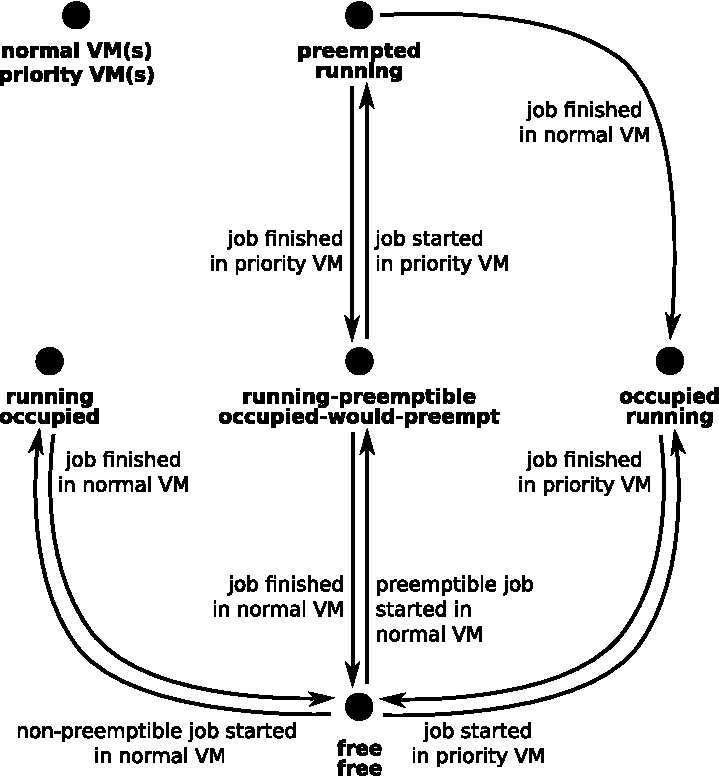
\includegraphics[width=.6\textwidth]{preemption}
    \end{center}
    \caption{States and transitions between them for preemptible
        virtual machines.}
    \label{fig:preemption}
\end{figure}

In the current implementation, only single-node jobs are considered as
preemptible (technically there is no need for such limitation, but the
scheduler had to be changed much more extensively to support this behavior
correctly). When a non-preemptible job is running in normal domain, its status
is \textit{running} and high-priority domain is in \textit{occupied} state and
no jobs can be submitted to this domain. However, if a preemptible job is
running in a normal domain, its state is \textit{running-preemptible} and
status of privileged domain is \textit{occupied-would-preempt}. In this case,
when a job is started in the privileged domain, status of the normal domain is
changed to \textit{preempted}.

To avoid starvation of preemptible jobs, Magrathea status contains not only
status information, but also \textit{length of preemption}, which is a number
of seconds jobs were preempted aggregated for each virtual node.  This length
of preemptions is used when scheduler selects new domain to be preempted.

While in the previous case no modification of PBS was necessary, in this case
PBS scheduler must be changed:

\begin{itemize}

\item Scheduler reads Magrathea status from the cache and schedules jobs with
respect to the domain status. A job can be submitted only to domains with
status \emph{free}, \emph{running}, \emph{occupied-would-preempt} and
\emph{running-preemptible}.

\item When the scheduler has more than one node capable to run a job, nodes
are sorted using length of preemption. The scheduler prefers nodes which will
not preempt jobs and if not available, the scheduler will prefer nodes with
the smallest length of preemption.

\item For parallel jobs, PBS Mom was modified to run different
prologue/epilogue scripts on all nodes. In standard PBS, prologue/epilogue
scripts are started only on the first node.

\item When the slave reports job startup to the master, more information about
job is published (number of CPUs and nodes used by the job).

\item Queue dedicated to parallel jobs was created, with several constraints:

    \begin{itemize}

    \item Jobs from this queue could be submitted only to high-priority nodes,
    not to preemptible nodes (nodes without Magrathea instalation can be used
    too).

    \item Only limited number of parallel jobs can be started in the same
    time, by the same user etc.

    \end{itemize}

\item When a domain is going to be preempted, the Magrathea slave daemon may
suspend jobs if needed. In the current version, the slave checks memory usage
of jobs. If there is danger that the machine will swap extensively after the
memory is reduced, the slave will send the SIGSTOP signal to all processes
belonging to suspended jobs. When the domain becomes active again, the slave
resumes all suspended jobs using the SIGCONT signal.

\end{itemize}


\subsection{More Than Two Running Domains}

Previous two use-cases can be combined, leading to the scenario where more
than two domains are ready to run jobs and a subset of these domains can
preempt remaining domains. With the limitation that at most one non-privileged
domain can run jobs and at most one preempting domain can be active, there is
no need for further modifications. In such a case, all high-priority VMs are
marked as \emph{free} or \emph{occupied-would-preempt} as long as none of them
is running any job. When a job which is allowed to preempt other jobs arrives
to a high-priority VM, the state of the virtual machine which has been marked
as \emph{running-preemptible} (if there is such a VM) is changed to
\emph{preempted}. States of other high-priority VMs are turned to
\emph{occupied} so that no other job is allowed to be submitted on the
particular worker node. When the privileged job finishes, the preempted
virtual machine is returned back into \emph{running-preemptible} and all
high-priority VMs are marked as \emph{occupied-would-preempt}.

To allow several virtual machines running jobs at the same time, Magrathea has
been enhanced to support CPU counting. This setup is used on our 16~core
machines, when it is not suitable to dedicate whole physical machine to one
virtual machine only. During job startup, the slave reports to the master
number of CPUs used by this job. Master can recompute states of all virtual
machines, together with counters of CPUs used by each job in all virtual
machines and also number of free, not allocated, CPUs. Magrathea status
contains not only state information and length of preemption, but also number
of CPUs allocated for this domain and number of free CPUs available for new
jobs submitted to this domain. PBS scheduler must be modified to use this
number of free CPUs instead of the one reported by PBS Mom.

This setup can be combined with preemption scenario, where subset of domains
is marked as high-priority domains, which are able to preempt standard
domains. Each CPU can be either free, used by a running job, or available only
for high-priority domains as it was occupied by a virtual machine which has
been preempted. When a job is submitted into a virtual machine (either normal
or high-priority), CPUs required by the job are taken from a set of free CPUs.
If the number of free CPUs is not large enough to satisfy the job and the job
was submitted into a high-priority virtual machine, a master daemon tries to
use CPUs which were occupied by preempted virtual machines. Only when those
CPUs cannot satisfy the job, another virtual machine is preempted. In other
words, normal and high-priority virtual machines can be running jobs at the
same time as long as high-priority jobs do not require all CPUs of a
particular node. When a job finishes, the master daemon tries to find and
resume a preempted virtual machine which would be satisfied with the CPUs that
are no longer occupied by the job. Thus CPUs are marked as free only when no
virtual machine could make use of them.

In this case we use only CPU counting as memory requirements are hard to
obtain before a job is actually started. Because of this, CPU counting is
really useful only for virtual machine monitors which support dynamic sharing
of memory between virtual machines, such as VServer. Using Xen would require
static partitioning of physical memory among all running virtual machines.

A set of states is the same as in the previous case, i.e., \textit{free},
\textit{running}, \textit{running-preemptible}, \textit{occupied},
\textit{occupied-would-preempt}, and \textit{preempted}. Normal virtual
machines are \emph{free} when at least one CPU is free, otherwise they are
\emph{occupied}. High-priority VMs are \emph{free} only when at least one CPU
is free and no virtual machine which can be preempted is running. If a
preemptible virtual machine is running, all high-priority VMs are in
\emph{occupied-would-preempt} state to stress the possibility that submitting
a job into such VM may result in preempting another VM. A virtual machine is
\emph{occupied} when no CPU (either free or freed by preemption) is available
for this VM.

Because set of states is identical to the previous use-case, the only change
in the PBS setup is a modification of PBS scheduler, which must use number of
free CPUs from Magrathea status.

\subsection{Frozen Services}

The last use-case described in this report deals with suspended virtual
domains in Xen. This is a case of services, started by user, running for short
time and then suspended by user request. When service is later needed, this
domain can be repeatedly resumed for a short time to perform a high-priority
computation.

Ability to suspend virtual machine adds one more state: \textit{frozen}. In
the current implementation, jobs which can be suspended are submitted to
domains which behave similarly to high-priority domains in preemption
scenario. When service domain is suspended (frozen), preemptible jobs can be
submitted to the normal domain, but when frozen domain becomes active again
(is resumed), normal domain is preempted (Figure~\ref{fig:frozen}).

\begin{figure}[tb]
    \begin{center}
    
\includegraphics[width=.8\textwidth]{frozen}
    \end{center}
    \caption{States and transitions between them for frozen
        virtual machines.}
    \label{fig:frozen}
\end{figure}

Magrathea has to be extended to support suspend/resume commands. Suspend
command can be initiated either by the owner of job or by the administrator.
Similarly, resume command can be issued by the user of suspended job or by the
administrator. Both commands are interpreted by master daemon. Proper
authorization has to be finished yet. Currently we support only limited
authorization, when only job owner or the administrator can suspend or resume
a domain, and only if one job is running in this domain.

On the PBS side, support for frozen domains require larger adaptation of PBS
when comparing with previous examples, because in this case also PBS server
must be modified. In opposite to all other types of domains, suspended domains
are not accessible and PBS Mom cannot response to monitoring requests from PBS
server.  Therefore we had to modify PBS server to check Magrathea status of
domains too and in case of suspended domains, monitoring of these domains is
deactivated.

\section{Related Work}

Interesting features of virtual machines inspired several projects with aims
similar to Magrathea. Motivation for a project of physicists in
Karlsruhe~\cite{karlsruhe}, sharing cluster between groups of users with
different requirements, is very alike to our first use. Although the initial
motivation was the same, their approach is different; they developed
standalone service, managing jobs and nodes of cluster.  If job is planned to
be started, new virtual machine corresponding to jobs is created by this
service. This approach is difficult to implement as it ends up with
reimplementing most parts of batch queuing system within the daemon. 

Integration of Xen virtual machine monitor, Moab scheduler, and Torque
resource management system was described in DVC~\cite{dvc}. With help of Moab
developers authors managed to provide transparent creation of clusters of
virtual machines. Virtual clusters are also allowed to span multiple physical
clusters by borrowing required resources from resource managers of the other
clusters. Main difference between DVC and Magrathea approach is a level of
integration. DVC is tightly integrated with Moab/Torque and it also integrates
image management system so that each virtual machine is started from an image
required by a job for which the virtual machine is being created. As virtual
machines in DVC are created and destroyed dynamically, a lot of work had to be
done to assure correct registration of new resources at all relevant parts of
the system. Results based of this approach were demonstrated also in a
presentation~\cite{chep07}, where different Xen based virtual machines were
used to run ATLAS (grid) and WestGrid (local) jobs, while parallel MPI jobs
were running in non-virtualized environment.

In our approach, Magrathea does not cover management of system images for
virtual machines and we do not expect a batch system to do this job either.
Instead, existing systems, such as Virtual Workspaces~\cite{workspaces} or
In-VIGO~\cite{invigo}, can be used for that purpose. This separation not only
simplifies the design of Magrathea but also makes sharing resources among
several batch systems easier as it reduces the number of changes to those
batch systems.


\section{Conclusions and Future Work}

In this report, we have described system Magrathea, which allows us to run
virtual nodes on a cluster. Nodes are managed by slightly modified PBS Pro.
Magrathea provides possibility to run different Linux flavors on one cluster
node and switch between them dynamically, gives us possibility to preempt
sequential jobs and therefore improves support for large parallel jobs on our
cluster. We have also described two new extensions, providing ability to run
several active domains concurrently on VServer enabled nodes and ability to
suspend jobs on Xen enabled clusters. Magrathea is deployed in production
environment on computational nodes of \META{Center}. First two described
scenarios are used in production, providing sharing worker nodes between
\META{Center} and EGEE and improved support for parallel jobs. Next two
scenarios will be deployed in production after current implementation is
verified by more extensive tests.

The overhead of Magrathea can be observed when jobs are started or stopped. We
have made some measurements on our production cluster using Xen virtual
machine monitor and the overhead of Magrathea showed to be negligible
concerning the time consumed by a job itself. When a job is being started,
Magrathea needs about 1.2 seconds to verify the request and to assign memory
and CPU power to a particular virtual machine. When another virtual machine
was previously running, memory must first be removed from it. This takes
additional time, which depends on the amount of data that has to be swapped
out to free occupied memory. In case no job is running in the second virtual
machine, it takes approx. 2.6 seconds to reassign the memory. Virtual machines
which are not running any jobs get only a small amount of CPU power, so that
running jobs are not slowed down. However, reduced CPU power does not have
serious impact on responsiveness of idle virtual machines. They are still able
to answer requests from PBS server. We have measured this using a standard
\texttt{ping} tool. Round-trip-time varies more for idle virtual machine with
restricted access to CPU power, but it is still negligible. The values are
(minimum RTT, average RTT, maximum RTT, standard deviation) 0.3~ms, 0.5~ms,
0.7~ms, 0.1~ms for running virtual machine and 0.2~ms, 6.0~ms, 87.4~ms,
15.5~ms for idle VM.

The implementation is general enough to support both VServer and Xen virtual
machine implementations. Even if Magrathea is currently supported only by our
PBS Pro modifications, we believe that at least first three use cases could be
easily integrated with other resource management systems too.

In future work, we would like to investigate migration of virtual domains and
enhance Magrathea to support such use-case. We also started cooperation with
researchers in scheduling area to develop new scheduler, which will be able to
utilize benefits provided by virtualization, especially preemption and
migration.

\section*{Acknowledgments}

This project has been supported by research intents ``Optical Network of
National Research and Its New Applications'' and ``Parallel and Distributed
Systems'' (M\v{S}M 6383917201, M\v{S}M 0021622419).

\begin{thebibliography}{99}
\bibitem{dvc}
W. Emeneker, D. Jackson, K. Butikofer, D. Stanzione.
Dynamic Virtual Clustering with Xen and Moab.
In {\em Frontiers of High Performance Computing and Networking -- ISPA 2006
Workshops}, Springer-Verlag LNCS 4331, 2006.

\bibitem{workspaces}
K. Keahey, K. Doering, and I. Foster. From Sandbox to Playground: Dynamic
Virtual
Environments in the Grid. In: {\em 5th International Workshop in Grid Computing
(Grid 2004)}. 2004.

\bibitem{invigo}
S. Adabala, V. Chadha, P. Chawla, R. Figueiredo, J. Fortes, I. Krsul,
A. Matsunaga, M. Tsugawa, J. Zhang, M. Zhao, L. Zhu, X. Zhu.
From virtualized resources to virtual computing Grids: The In-VIGO system. Future Generation
Computer Systems 21,2005.

\bibitem{xen}
P. Barham, B. Dragovic, K. Fraser, S.
Hand, T. Harris, A. Ho, R. Neugebar, I. Pratt, and A.
Warfield. Xen and the Art of Virtualization. In {\em ACM
Symposium on Operating Systems Principles (SOSP)}. October 2003.

\bibitem{vserver}
Stephen Soltesz, Herbert Potzl, Marc E. Fiuczynski, Andy Bavier and Larry Peterson. Container-based
Operating System Virtualization: A Scalable, High-performance Alternative to Hypervisors. April 2007.
\url{http://wireless.cs.uh.edu/presentation/2006/07/Container.pdf}.

\bibitem{chep07} Sergey Chechelnitskiy. Running CE and SE in a Xen-virtualized environment. Presented on
CHEP 2007 conference.

\bibitem{vee} Ji\v{r}\'\i{} Denemark and Miroslav Ruda. Magrathea: Enabling New Applications Using Cluster
Virtualization. Submited to conference Virtual Execution Environments 2008.

\bibitem{ganglia}Matthew L. Massie, Brent N. Chun and David E. Culler.
The ganglia distributed monitoring system: design, implementation, and experience.
In Parallel Computing Volume 30, Issue 7. 2004. pages 817-840. 	

\bibitem{karlsruhe}
V. B\"uge, Y. Kemp, M. Kunze, O. Oberst, and G. Quast.
Virtualizing a Batch Queuing System at a University Grid Center.
In {\em Frontiers of High Performance Computing and Networking -- ISPA 2006
Workshops}, Springer-Verlag LNCS 4331, 2006.

\bibitem{vmms}
Mendel Rosenblum and Tal Garfinkel. Virtual Machine Monitors: Current Technology
and Future Trends. Computer, 38(5):3947, 2005.

\end{thebibliography}
\end{document}
